\documentclass{beamer}
\usepackage[utf8]{inputenc}
\usepackage{graphicx, epsfig}
\usepackage{amsmath,mathrsfs,amsfonts,amssymb}
%\usepackage{subfig}
\usepackage{floatflt}
\usepackage{epic,ecltree}
\usepackage{mathtext}
\usepackage{fancybox}
\usepackage{fancyhdr}
\usepackage{multirow}
\usepackage{enumerate}
\usepackage{epstopdf}
\usepackage{multicol}
\usepackage{algorithm}
\usepackage[noend]{algorithmic}
\def\algorithmicrequire{\textbf{Input:}}
\def\algorithmicensure{\textbf{Output:}}
\usetheme{default}%{Singapore}%{Warsaw}%{Warsaw}%{Darmstadt}
\usecolortheme{default}
\setbeamertemplate{footline}[page number]{}
\setbeamerfont{title}{size=\Huge}

\newcommand{\bt}{\mathbf{t}} 
\newcommand{\bu}{\mathbf{u}} 
\newcommand{\bw}{\mathbf{w}} 
\newcommand{\bx}{\mathbf{x}} 
\newcommand{\bz}{\mathbf{z}} 
\newcommand{\by}{\mathbf{y}} 

\newcommand{\bI}{\mathbf{I}} 
\newcommand{\bT}{\mathbf{T}} 
\newcommand{\bX}{\mathbf{X}} 
\newcommand{\bZ}{\mathbf{Z}} 

\newcommand{\bmu}{\boldsymbol{\mu}}
\newcommand{\bsigma}{\boldsymbol{\sigma}}

\newcommand{\btheta}{\boldsymbol{\theta}} 
\newcommand{\bphi}{\boldsymbol{\phi}} 

\DeclareMathOperator*{\argmin}{arg\,min}
\DeclareMathOperator*{\argmax}{arg\,max}

%\definecolor{beamer@blendedblue}{RGB}{15,120,80}
%----------------------------------------------------------------------------------------------------------
\title[\hbox to 56mm{Deep Generative Models  \hfill\insertframenumber\,/\,\inserttotalframenumber}]
{Deep Generative Models \\ Lecture 4}
\author[Roman Isachenko]{\\Roman Isachenko}
\institute[MIPT]{Moscow Institute of Physics and Technology \\
}
\date{2020}
%--------------------------------------------------------------------------------
\begin{document}
%--------------------------------------------------------------------------------
\begin{frame}
%\thispagestyle{empty}
\titlepage
\end{frame}
%--------------------------------------------------------------------------------
\subsection{Flow models}
\begin{frame}{Likelihood-based models so far...}
	\begin{minipage}[t]{0.5\columnwidth}
		\begin{block}{Autoregressive models}
			\vspace{-0.5cm}
			\[
			p(\bx|\btheta) = \prod_{i=1}^m p(x_i | \bx_{1:i - 1}, \btheta)
			\]
			\vspace{-0.2cm}
			\begin{itemize}
				\item tractable likelihood, 
				\item no inferred latent factors.
			\end{itemize}
		\end{block}
	\end{minipage}%
	\begin{minipage}[t]{0.5\columnwidth}
		\begin{block}{Latent variable models}
			\[
			p(\bx| \btheta) = \int p(\bx, \bz | \btheta) d \bz
			\]
			\begin{itemize}
				\item latent feature representation, 
				\item intractable likelihood.
			\end{itemize}
		\end{block}
	\end{minipage}
	
	\vspace{1cm } 
	How to build model with latent variables and tractable likelihood?
\end{frame}
%=======
\begin{frame}{Flows intuition}
	Let $X$ be a random variable with density $p_X(x)$. Then
	\[
	Z = F(X) = \int_{-\infty}^x p(t)dt \sim U[0, 1].
	\]
	Hence
	\[
	Z \sim U[0, 1]; \quad X = F^{-1}(Z) \quad X \sim p(x).
	\]
	\begin{figure}
		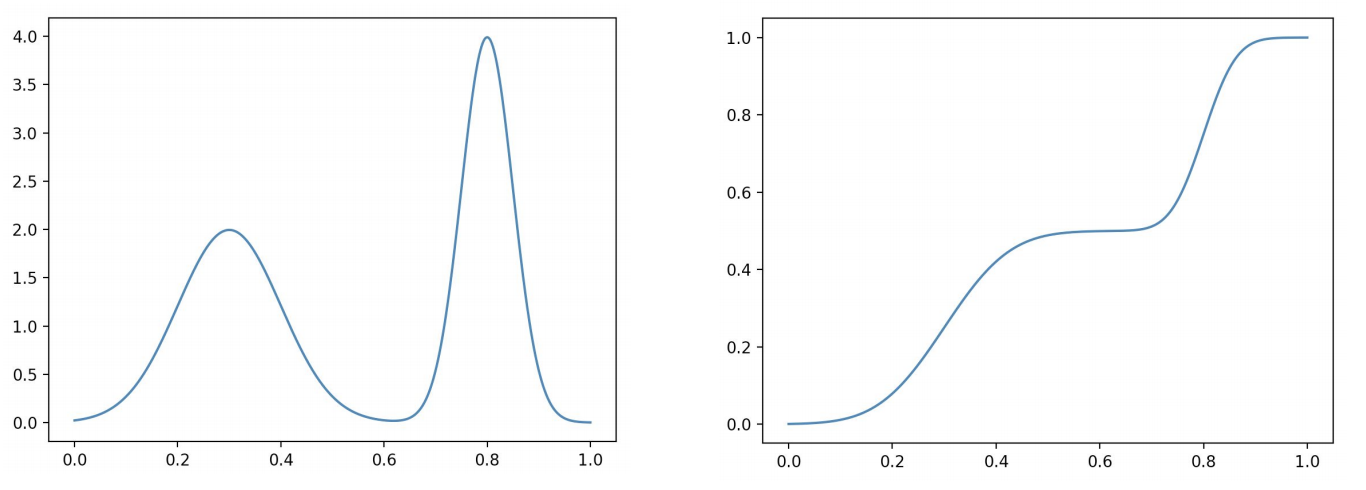
\includegraphics[width=\linewidth]{figs/flows_1d}
	\end{figure}
	
	\vfill
	\hrule\medskip
	{\scriptsize \href{https://sites.google.com/view/berkeley-cs294-158-sp19/home}{https://sites.google.com/view/berkeley-cs294-158-sp19/home}}
	
\end{frame}
%=======

\begin{frame}{Change of variables}
	\begin{block}{Theorem}
		Let 
		\begin{itemize}
			\item $\bx$ is a random variable, 
			\item $f: \mathbb{R}^m \rightarrow \mathbb{R}^m$ is a differentiable, invertible function,
			\item $\bz = f(\bx)$, $\bx = f^{-1}(\bz) = g(\bz)$.
		\end{itemize}
		Then
		\[
		p(\bx) = p(\bz) \left|\det \left(  \frac{\partial \bz}{\partial \bx} \right) \right| = p(f(\bx)) \left|\det \left(  \frac{\partial f(\bx)}{\partial \bx} \right) \right|.
		\]
	\end{block}
	\begin{block}{Note}
		\begin{itemize}
			\item $\bx$ and $\bz$ have the same dimensionality;
			\item $ \left|\det \left(  \frac{\partial f(\bx)}{\partial \bx} \right)\right| = \left|\det \left(  \frac{\partial g^{-1}(\bx)}{\partial \bx} \right)\right| = \left|\det \left(  \frac{\partial g(\bz)}{\partial \bz} \right)\right|^{-1}$;
			\item $f(\bx, \btheta)$ could be parametric.
		\end{itemize}
	\end{block}
\end{frame}
%=======
\begin{frame}{Flows}
\begin{figure}
	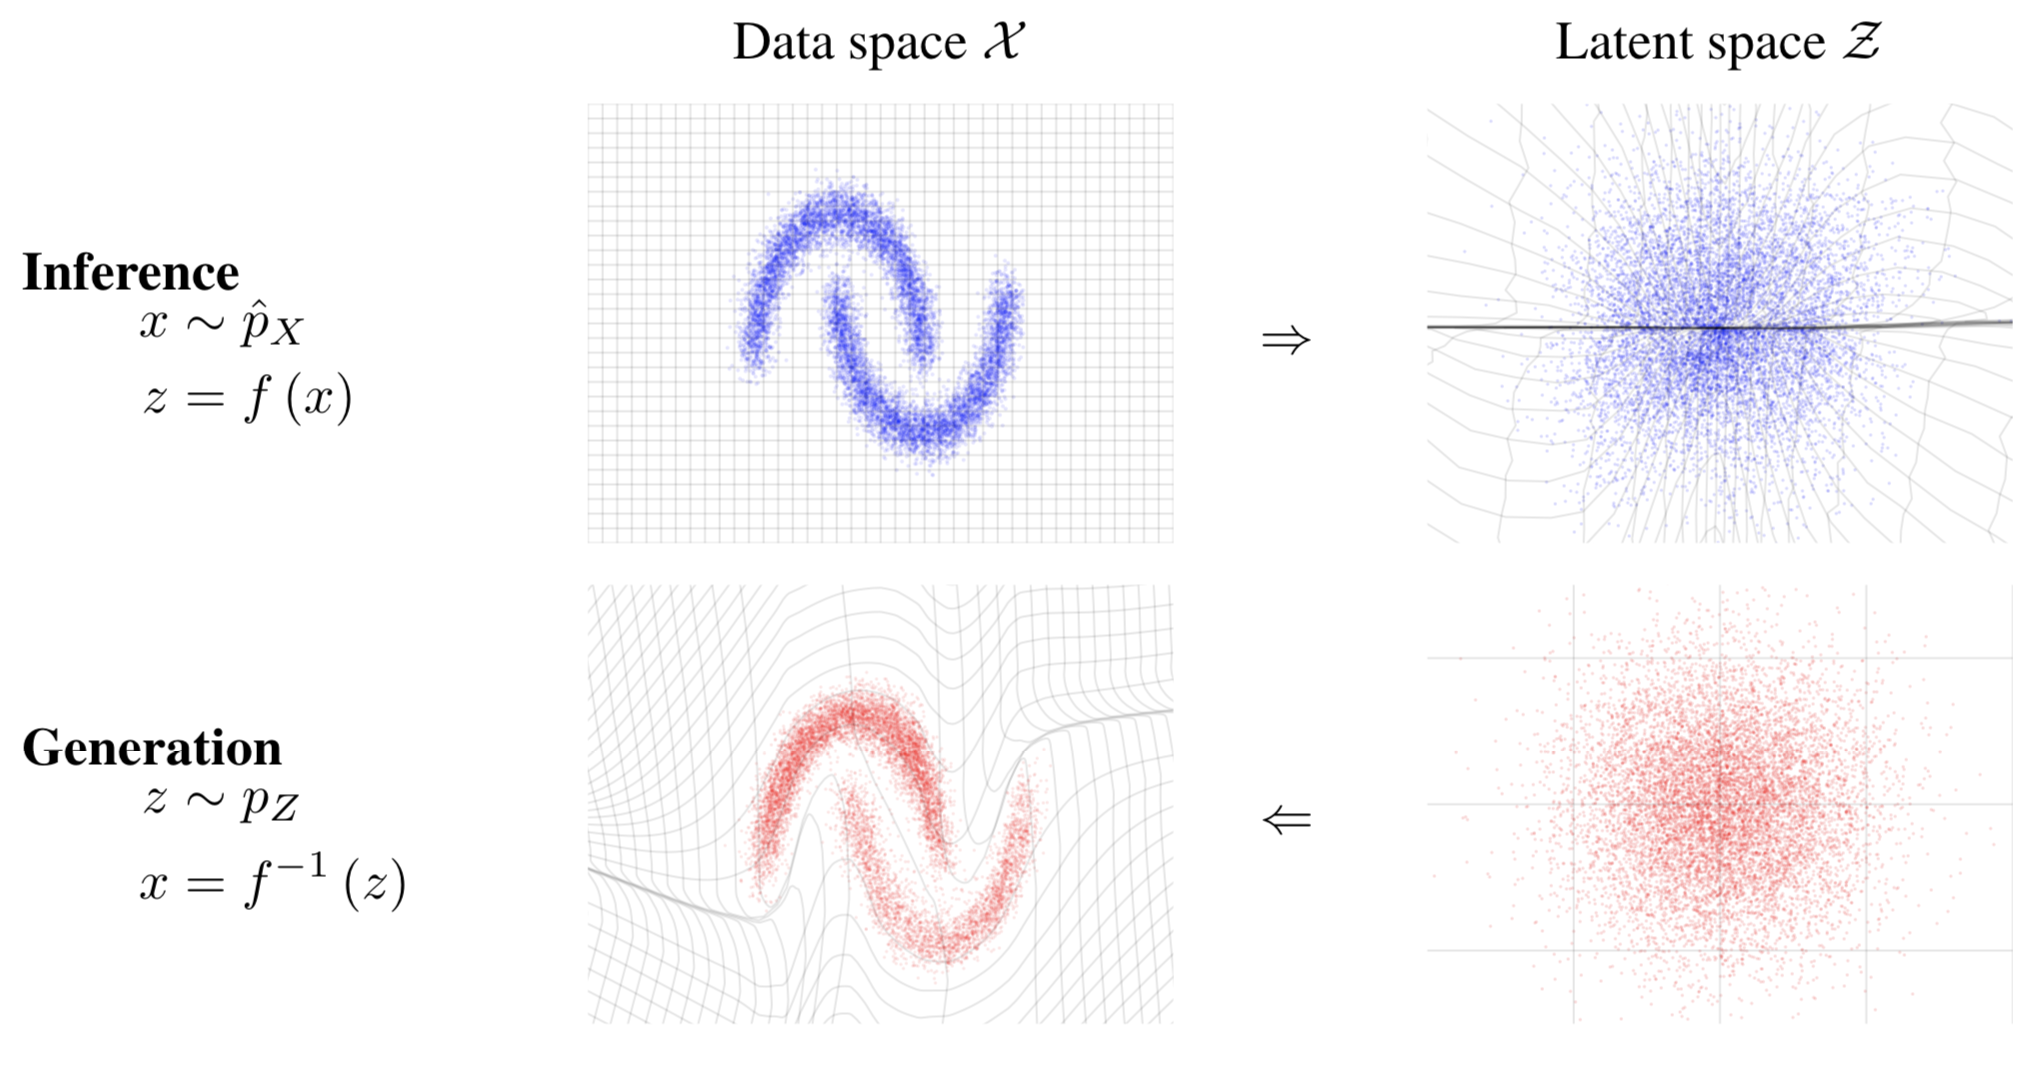
\includegraphics[width=0.8\linewidth]{figs/flows_how2.png}
\end{figure}
\begin{itemize}	
	\item Latent representation is given by $\bz = f(\bx, \btheta)$.
	\item Likelihood is given by $\bz = f(\bx, \btheta)$ and change of variables.
	\item Sampling of $\bx$ is performed by sampling from a base distribution $p(\bz)$ and applying $\bx = f^{-1}(\bz, \btheta) = g(\bz, \btheta)$.
\end{itemize}
\vfill
\hrule\medskip
{\scriptsize \href{https://arxiv.org/pdf/1605.08803.pdf}{https://arxiv.org/pdf/1605.08803.pdf}} 
\end{frame}
%=======
\begin{frame}{Fitting flows}
	\begin{block}{MLE problem}
		\vspace{-0.3cm}
		\[
		\btheta^* = \argmax_{\btheta} p(\bX | \btheta) = \argmax_{\btheta} \prod_{i=1}^n p(\bx_i | \btheta) = \argmax_{\btheta} \sum_{i=1}^n \log p(\bx_i | \btheta).
		\]
		\vspace{-0.3cm}
	\end{block}
	\begin{block}{Challenge}
		$p(\bx | \btheta)$ could be intractable.
	\end{block}
	\begin{block}{Fitting flow to solve MLE}
		\[
		p(\bx|\btheta) = p(\bz) \left|\det \left(  \frac{\partial \bz}{\partial \bx} \right) \right|  = p(f(\bx, \btheta)) \left|\det \left( \frac{\partial f(\bx, \btheta)}{\partial \bx} \right) \right|
		\]
	\end{block}
\end{frame}
%=======
\begin{frame}{Stacking flows}
	Let $\bz = f(\bx) = f_2 \circ f_1(\bx)$ and $f_1, f_2$ satisfy conditions of change of variable theorem (differentiable and invertible).
	\begin{multline*}
		p(\bx) = p(\bz) \left|\det \left(  \frac{\partial \bz}{\partial \bx} \right) \right| = p(f(\bx)) \left|\det \left(  \frac{\partial f(\bx)}{\partial \bx} \right) \right| = \\
		= p(f(\bx)) \left|\det \left(\frac{\partial f_2 \circ f_1(\bx)}{\partial \bx} \right) \right| =
		p(f(\bx)) \left|\det \left(\frac{\partial \textbf{f}_2}{\partial \textbf{f}_1} \cdot \frac{\partial \textbf{f}_1}{\partial \bx} \right) \right| = \\
		= p(f(\bx))  \left|\det \left(\frac{\partial \textbf{f}_2}{\partial \textbf{f}_1} \right) \right| \cdot \left| \det \left( \frac{\partial \textbf{f}_1}{\partial \bx} \right) \right|
	\end{multline*}

	What we will get in the case $\bz = f(\bx) = f_n \circ \dots \circ f_1(\bx)$?
\end{frame}
%=======
\begin{frame}{Flows}
	\[
	\log p(\bx|\btheta) = \log p(f(\bx, \btheta)) + \log \left|\det \left( \frac{\partial f(\bx, \btheta)}{\partial \bx} \right) \right|
	\]
	\begin{block}{Definition}
		Normalizing flow is a \textit{differentiable, invertible} mapping from data $\bx$ to the noise $\bz$. 
	\end{block}
	\begin{itemize}
		\item Normalizing - convert data distribution to \textit{noise}.
		\item Flow - sequence of such mapping is also a flow
		\[
		\bz = f_K \circ \dots \circ f_1(\bx); \quad \bx = f_1^{-1} \circ \dots \circ f_K^{-1} (\bz) = g_1 \circ \dots \circ g_K(\bz) 
		\] 
		\begin{multline*}
			p(\bx) = p(f_K \circ \dots \circ f_1(\bx)) \left|\det \left(\frac{\partial f_K \circ \dots \circ f_1(\bx)}{\partial \bx} \right) \right| = \\
			= p(f_K \circ \dots \circ f_1(\bx)) \prod_{k=1}^K \left|\det \left(\frac{\partial \mathbf{f}_k}{\partial \mathbf{f}_{k-1}} \right) \right|.
		\end{multline*}
	\end{itemize}
\end{frame}
%=======
\begin{frame}{Flows}
	\[
	\log p(\bx|\btheta) = \log p(f(\bx, \btheta)) + \log \left|\det \left( \frac{\partial f(\bx, \btheta)}{\partial \bx} \right) \right|
	\]
	What is the computational comprexity of computing the determinant?
	\begin{block}{What we want}
		\begin{itemize}
			\item Efficient computation of Jacobian $\frac{\partial f(\bx, \btheta)}{\partial \bx}$;
			\item Efficient sampling from the base distribution $p(\bz)$;
			\item Easy to invert $f(\bx, \btheta)$.
		\end{itemize}
		
	\end{block}
	
\end{frame}
%=======
\begin{frame}{Planar Flows, 2015}
	\vspace{-0.2cm}
	\[
	g(\bz, \btheta) = \bz + \mathbf{u} h(\bw^T\bz + b).
	\]
	\vspace{-0.2cm}
	\begin{itemize}
		\item $\btheta = \{\bu, \bw, b\}$;
		\item $h$ is a smooth element-wise non-linearity.
	\end{itemize}
	\begin{align*}
		\left| \det \left( \frac{\partial g(\bz, \btheta)}{\partial \bz} \right)\right| &= \left| \det \left( \bI +  h'(\bw^T \bz + b) \bw\bu^T\right) \right| \\
		&= \left| 1 + h'(\bw^T \bz + b) \bw^T \bu \right|
	\end{align*}
	The transformation is invertible if (just one of example)
	\[
	h = \tanh; \quad h'(\bw^T \bz + b) \bu^T \bw \geq -1.
	\]
	\vfill
	\hrule\medskip
	{\scriptsize \href{https://arxiv.org/pdf/1505.05770.pdf}{https://arxiv.org/pdf/1505.05770.pdf}} 
\end{frame}
%=======
\begin{frame}{Planar Flows, 2015}
	\[
	\bz_K = g_1 \circ \dots \circ g_K (\bz); \quad g_k = g(\bz_k, \btheta_k).
	\]
	\begin{figure}
		\centering
		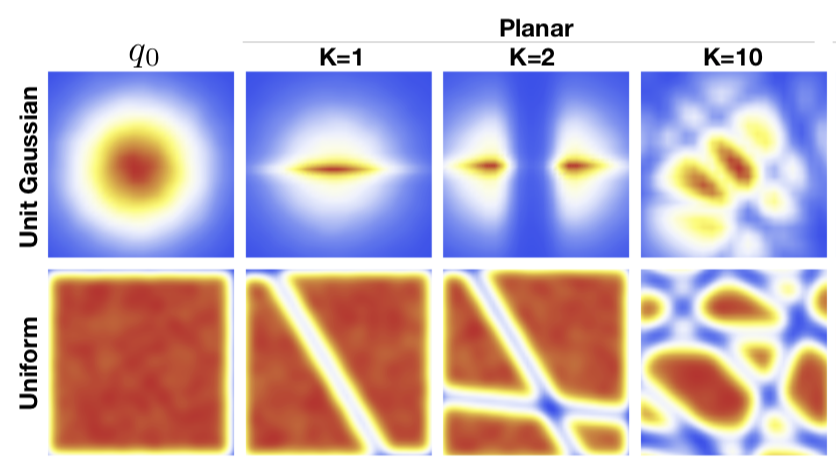
\includegraphics[width=0.9\linewidth]{figs/planar_flows.png}
	\end{figure}
	\vfill
	\hrule\medskip
	{\scriptsize \href{https://arxiv.org/pdf/1505.05770.pdf}{https://arxiv.org/pdf/1505.05770.pdf}} 
\end{frame}
%=======
\begin{frame}{Jacobian structure}
	\begin{itemize}
		\item What is the determinant of a diagonal matrix?
		\[
		\bz = f(\bx, \btheta) = (f_1(x_1, \btheta), \dots, f_m(x_m, \btheta)).
		\]
		\[
		\log \left|\det \left( \frac{\partial f(\bx, \btheta)}{\partial \bx} \right) \right| = \log \left| \prod_{i=1}^m f_i'(x_i, \btheta) \right| = \sum_{i=1}^m \log \left| f_i'(x_i, \btheta) \right|.
		\]
		\item What is the determinant of a triangular matrix? \\
		Let $z_i$ depends only on $\bx_{1:i}$ (or without loss of generality $x_i$ depends on $\bz_{1:i}$). \\
		What is the inverse of such transformations?
	\end{itemize}
\end{frame}
%=======
\begin{frame}{NICE, 2014}
	\begin{block}{Coupling layer}
		\begin{equation*}
			\begin{cases} \bz_{1:d} = \bx_{1:d} \\ \bz_{d:m} = \tau (\bx_{d:m}, c(\bx_{1:d}))\end{cases} \quad 
			\begin{cases} \bx_{1:d} = \bz_{1:d} \\ \bx_{d:m} = \tau^{-1} (\bz_{d:m}, c(\bz_{1:d}))\end{cases}
		\end{equation*}
		\begin{itemize}
			\item $c: \mathbb{R}^d \rightarrow \mathbb{R}^{k}$ -- coupling function;
			\item $\tau : \mathbb{R}^{m - d} \times c(\mathbb{R}^d) \rightarrow \mathbb{R}^{m - d}$ -- coupling law.
			\item 
			\[
			\det \left( \frac{\partial \bz}{\partial \bx} \right) = \det 
			\begin{pmatrix}
				\bI_d & 0_{d \times m - d} \\
				\frac{\partial \bz_{d:m}}{\partial \bx_{1:d}} & \frac{\partial \bz_{d:m}}{\partial \bx_{d:m}}
			\end{pmatrix} = 
			\det \left( \frac{\partial \bz_{d:m}}{\partial \bx_{d:m}} \right)
			\]
		\end{itemize}
	\end{block}
	\vfill
	\hrule\medskip
	{\scriptsize \href{https://arxiv.org/pdf/1410.8516.pdf}{https://arxiv.org/pdf/1410.8516.pdf}} 
\end{frame}
%=======
\begin{frame}{NICE, 2014}
	\begin{block}{Coupling layer}
		\vspace{-0.5cm}
		\begin{equation*}
			\begin{cases} \bz_{1:d} = \bx_{1:d}; \\ \bz_{d:m} = \tau (\bx_{d:m}, c(\bx_{1:d}));\end{cases} 
			\quad \Rightarrow \quad 
			\begin{cases} \bx_{1:d} = \bz_{1:d}; \\ \bx_{d:m} = \tau^{-1} (\bz_{d:m}, c(\bz_{1:d})).\end{cases}
		\end{equation*}
		\vspace{-0.5cm}
	\end{block}
	\begin{block}{Coupling function $c(\cdot)$}
		Any complex function (without restrictions). For example, neural network.
	\end{block}
	\begin{block}{Coupling law $\tau(\cdot, \cdot)$}
		\begin{itemize}
			\item $\tau(x, c) = x + c$ -- \textit{additive};
			\item $\tau(x, c) = x \odot c, \, c \neq 0$ -- multiplicative;
			\item $\tau(x, c) = x \odot c_1 + c_2, \, c_1 \neq 0$ -- affine.
		\end{itemize}
	\end{block}
	To obtain more flexible class of dictributions, stack more coupling layers (with different ordering of components!). \\
	
	\vfill
	\hrule\medskip
	{\scriptsize \href{https://arxiv.org/pdf/1410.8516.pdf}{https://arxiv.org/pdf/1410.8516.pdf}} 
\end{frame}
%=======
\begin{frame}{NICE, 2014}
	\[
	\det \left( \frac{\partial \bz}{\partial \bx} \right) = \det 
	\begin{pmatrix}
		\bI_d & 0_{d \times m - d} \\
		\frac{\partial \bz_{d:m}}{\partial \bx_{1:d}} & \frac{\partial \bz_{d:m}}{\partial \bx_{d:m}}
	\end{pmatrix} = 
	\det \left( \frac{\partial \bz_{d:m}}{\partial \bx_{d:m}} \right)
	\]
	What is the Jacobian for the additive coupling law $\tau(x + c) = x + c$? \\
	In this case the transformation is \textit{volume preserving}. \\
	The last layer is rescaling:
	\[
	z_i = s_i x_i; \quad x_i = z_i / s_i.
	\]
	What is the Jacobian of the last layer?
	\vfill
	\hrule\medskip
	{\scriptsize \href{https://arxiv.org/pdf/1410.8516.pdf}{https://arxiv.org/pdf/1410.8516.pdf}} 
\end{frame}
%=======
\begin{frame}{NICE, 2014}
	\begin{figure}
		\centering
		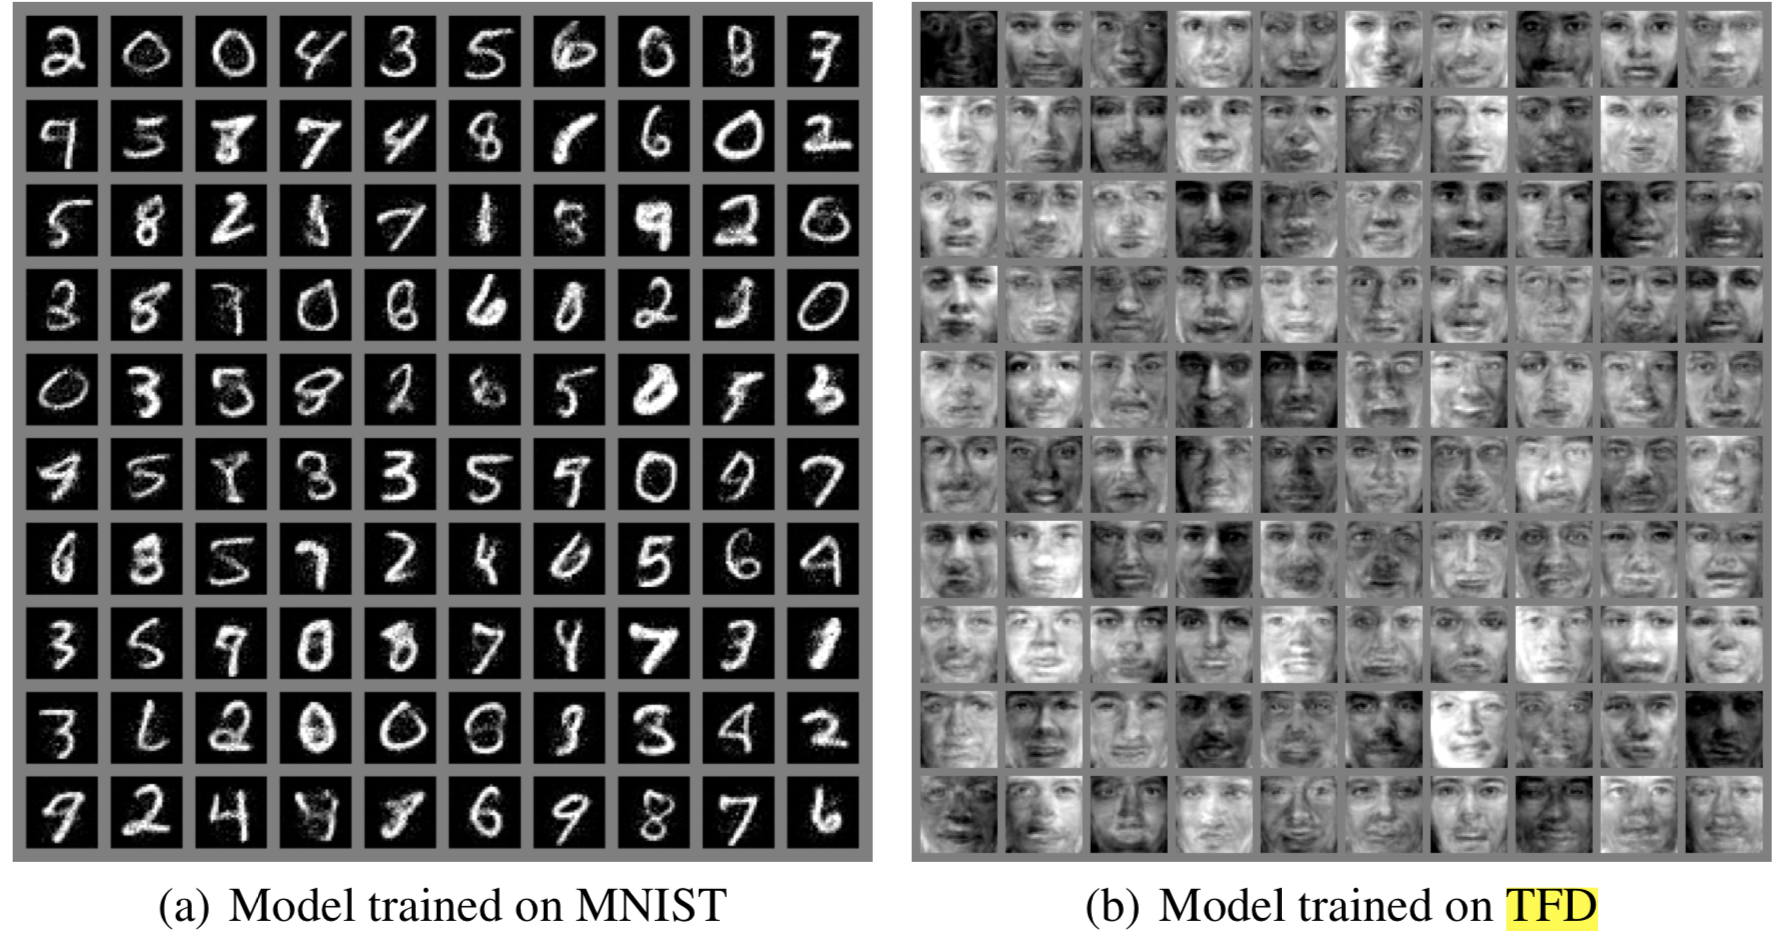
\includegraphics[width=\linewidth]{figs/nice.png}
	\end{figure}
	\vfill
	\hrule\medskip
	{\scriptsize \href{https://arxiv.org/pdf/1410.8516.pdf}{https://arxiv.org/pdf/1410.8516.pdf}} 
\end{frame}
%=======
\begin{frame}{RealNVP, 2016}
	\begin{block}{Affine coupling law}
		\[
		\begin{cases} \bz_{1:d} = \bx_{1:d}; \\ \bz_{d:m} = \bx_{d:m} \odot \exp \left(c_1(\bx_{1:d}, \btheta)\right) + c_2(\bx_{1:d}, \btheta).\end{cases} 
		\]
		\[
		\begin{cases} \bx_{1:d} = \bz_{1:d}; \\ \bx_{d:m} = \left(\bz_{d:m} - c_2(\bx_{1:d}, \btheta) \right) \odot \exp(-c_1(\bx_{1:d}, \btheta)).\end{cases}
		\]
	\end{block}
	\begin{block}{Jacobian}
		\vspace{-0.3cm}
		\[
		\det \left( \frac{\partial \bz}{\partial \bx} \right) = \det 
		\begin{pmatrix}
			\bI_d & 0_{d \times m - d} \\
			\frac{\partial \bz_{d:m}}{\partial \bx_{1:d}} & \frac{\partial \bz_{d:m}}{\partial \bx_{d:m}}
		\end{pmatrix} = \prod_{i=1}^{m - d} \exp (c_1(\bx_{1:d}, \btheta)_i).
		\]
		Non-Volume Preserving.
	\end{block}
	\vfill
	\hrule\medskip
	{\scriptsize \href{https://arxiv.org/pdf/1605.08803.pdf}{https://arxiv.org/pdf/1605.08803.pdf}} 
\end{frame}
%=======
\begin{frame}{RealNVP, 2016}
	\begin{figure}
		\centering
		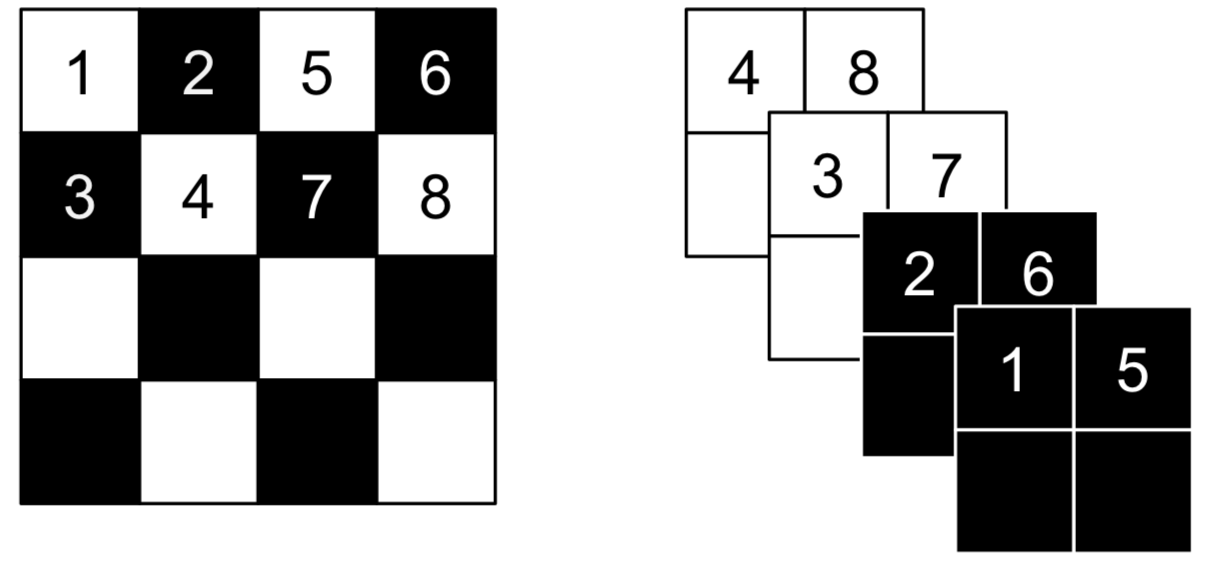
\includegraphics[width=0.75\linewidth]{figs/realnvp_masking.png}
	\end{figure}
	Masked convolutions are used to define ordering.
	\vfill
	\hrule\medskip
	{\scriptsize \href{https://arxiv.org/pdf/1605.08803.pdf}{https://arxiv.org/pdf/1605.08803.pdf}} 
\end{frame}
%=======
\begin{frame}{RealNVP, 2016}
	\begin{figure}
		\centering
		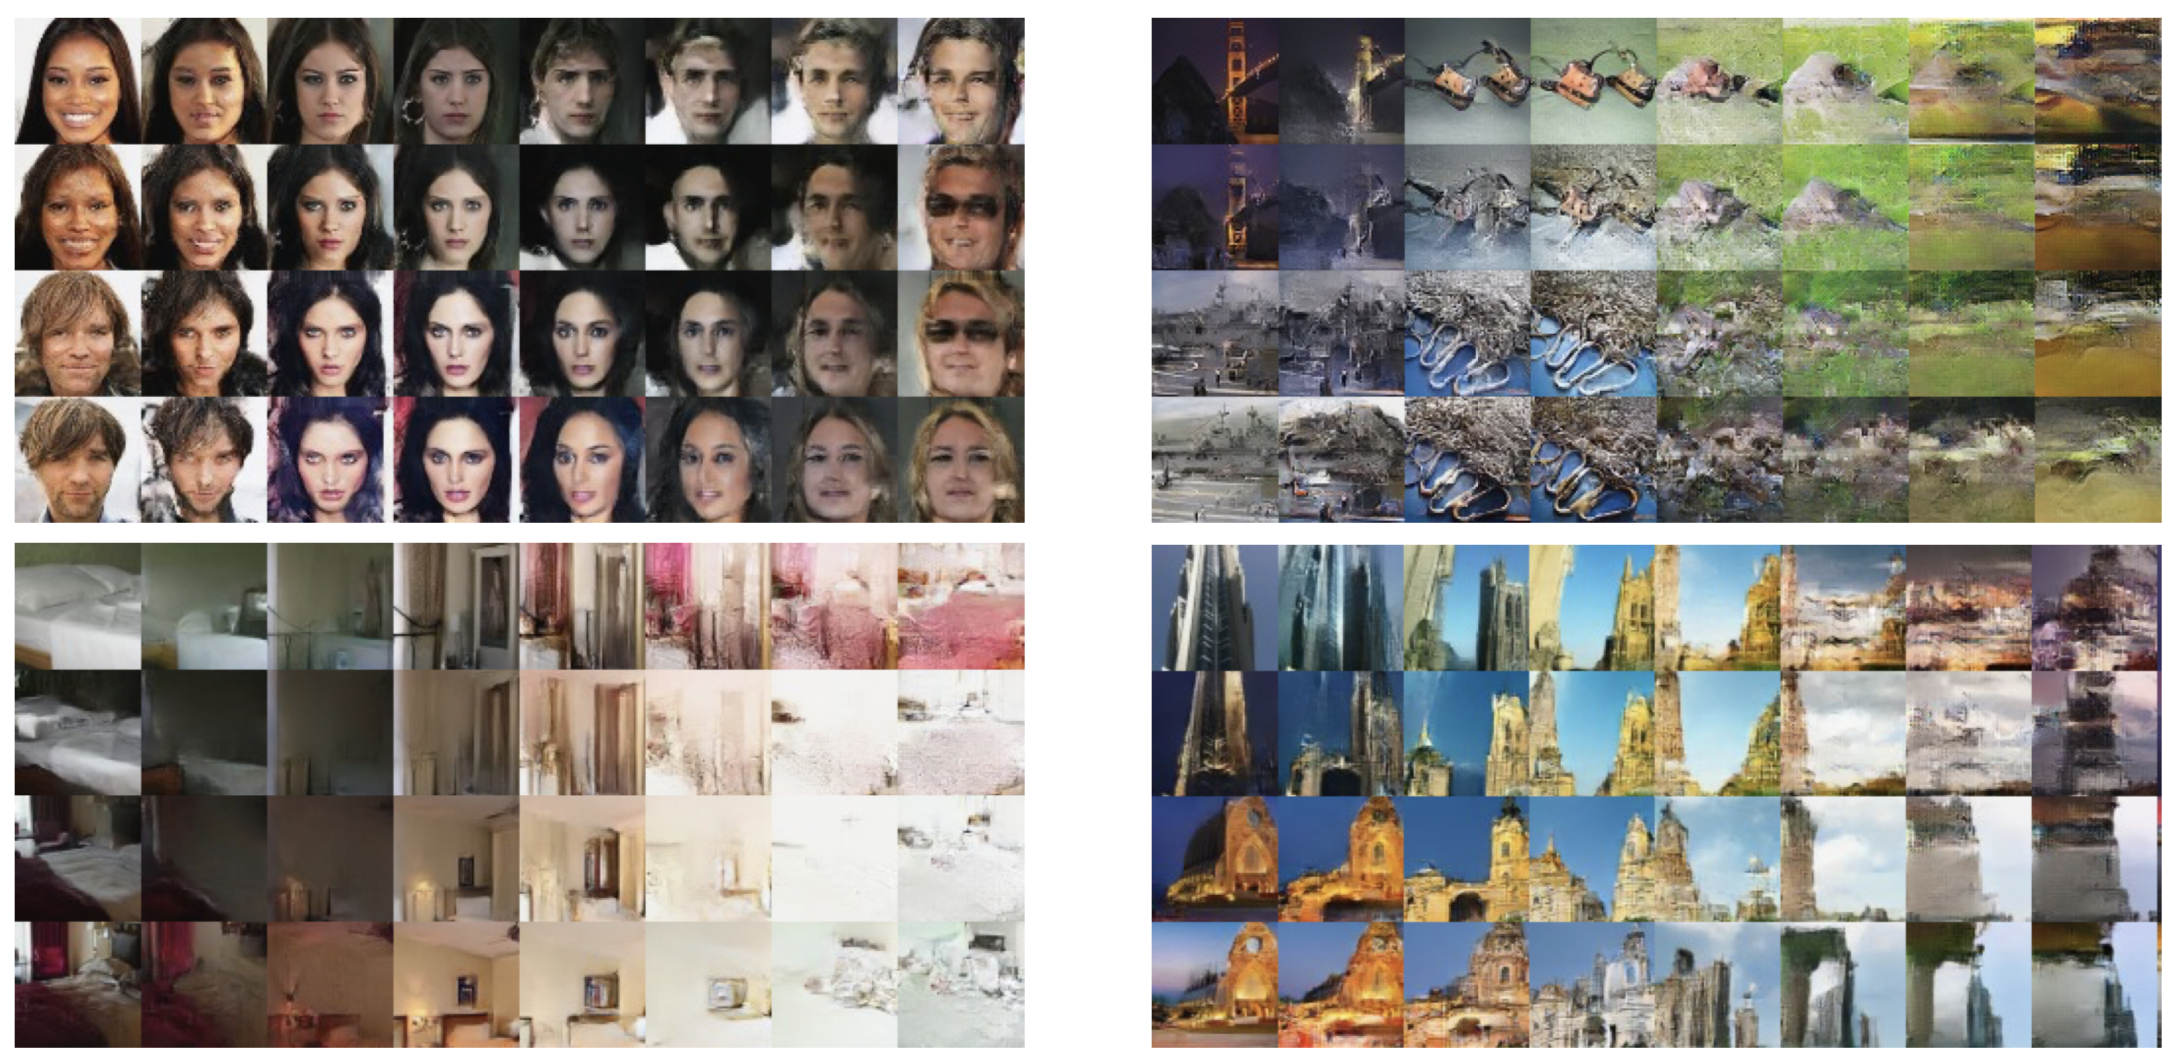
\includegraphics[width=\linewidth]{figs/realnvp_output.png}
	\end{figure}
	\vfill
	\hrule\medskip
	{\scriptsize \href{https://arxiv.org/pdf/1605.08803.pdf}{https://arxiv.org/pdf/1605.08803.pdf}} 
\end{frame}
%=======
\begin{frame}{RevNets, 2017}
	\begin{minipage}[t]{0.6\columnwidth}
		\begin{itemize}
			\item Modern neural networks are trained via backpropagation.
			\item Residual networks are state of the art in image classification.
			\item Backpropagation requires storing the network activations.
		\end{itemize}
	\end{minipage}%
	\begin{minipage}[t]{0.4\columnwidth}
		\begin{figure}
			\centering
			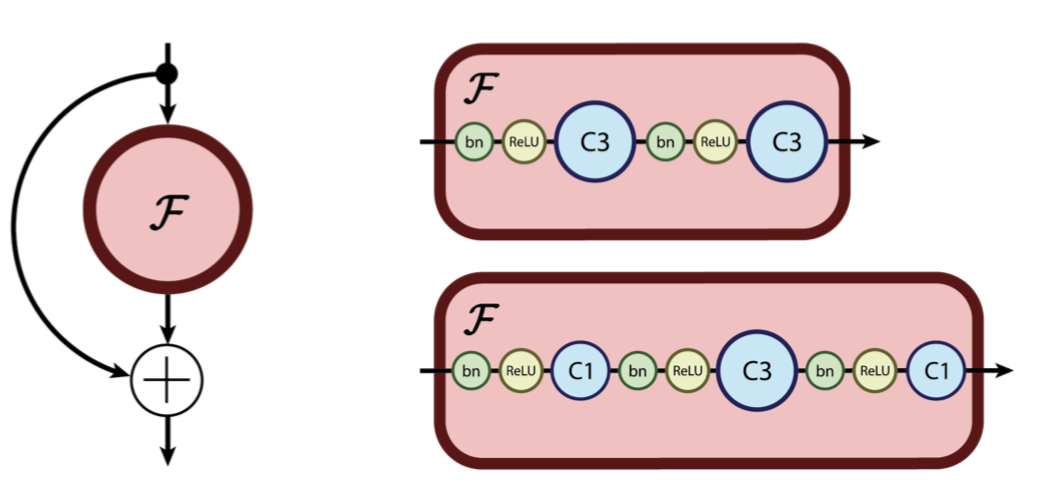
\includegraphics[width=\linewidth]{figs/resnet_block.png}
		\end{figure}
	\end{minipage}
	\vspace{0.1cm}
	\begin{block}{Problem}
		Storing the activations imposes an increasing memory burden. GPUs have limited memory capacity, leading to constraints often exceeded by state-of-the-art architectures (with thousand layers).
	\end{block}
	\vfill
	\hrule\medskip
	{\scriptsize \href{https://arxiv.org/pdf/1707.04585.pdf}{https://arxiv.org/pdf/1707.04585.pdf}} 
\end{frame}
%=======
\begin{frame}{RevNets, 2017}
	\begin{block}{NICE}
		\vspace{-0.2cm}
		\begin{equation*}
			\begin{cases} \bz_1 = \bx_1; \\ \bz_2 = \bx_2 + \mathcal{F}(\bx_1, \btheta);\end{cases}  \quad \Leftrightarrow \quad 
			\begin{cases} \bx_1 = \bz_1; \\ \bx_2 = \bz_2 - \mathcal{F}(\bz_1, \btheta).\end{cases} 
		\end{equation*}
		\vspace{-0.2cm}
	\end{block}
	\begin{block}{RevNet}
		\begin{equation*}
			\begin{cases} \by_1 = \bx_1 + \mathcal{F}(\bx_2, \btheta); \\ \by_2 = \bx_2 + \mathcal{G}(\by_1, \btheta);\end{cases} \quad \Leftrightarrow \quad 
			\begin{cases} \bx_2 = \by_2 - \mathcal{F}(\by_1, \btheta); \\ \bx_1 = \by_1 - \mathcal{G}(\bx_2, \btheta).\end{cases} 
		\end{equation*}
	\end{block}
	\begin{figure}
		\centering
		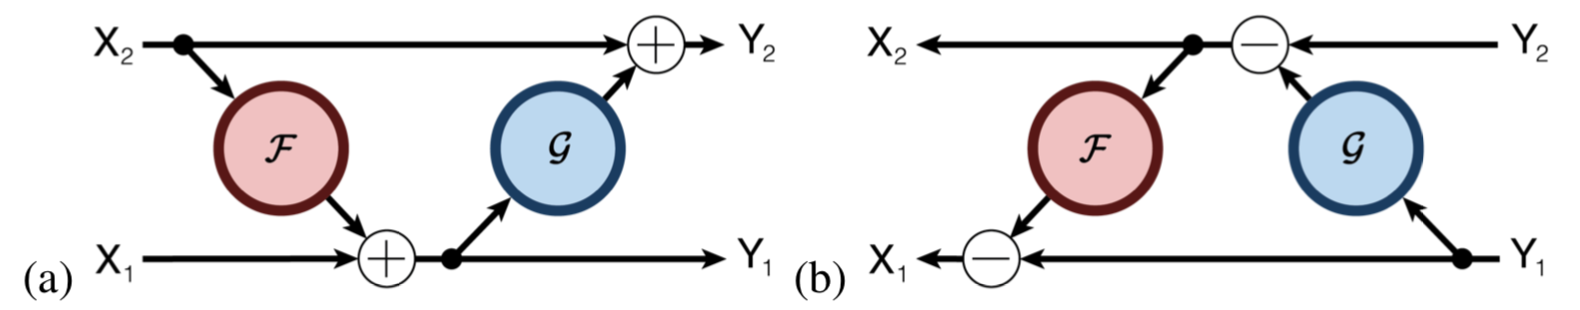
\includegraphics[width=\linewidth]{figs/revnet.png}
	\end{figure}
	\vfill
	\hrule\medskip
	{\scriptsize \href{https://arxiv.org/pdf/1707.04585.pdf}{https://arxiv.org/pdf/1707.04585.pdf}} 
\end{frame}
%=======
\begin{frame}{RevNets, 2017}
	\begin{figure}
		\centering
		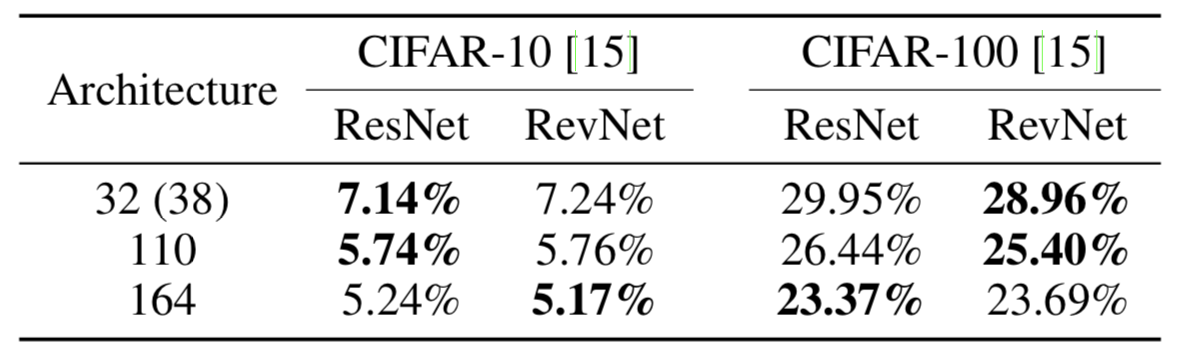
\includegraphics[width=0.8\linewidth]{figs/revnet_results.png}
	\end{figure}
	\begin{itemize}
		\item If the network contains non-reversible blocks (poolings, strides), activations for this blocks should be stored.
		\item To avoid storing activations in the modern frameworks, the backward pass should be manually redefined.
	\end{itemize}
	\vfill
	\hrule\medskip
	{\scriptsize \href{https://arxiv.org/pdf/1707.04585.pdf}{https://arxiv.org/pdf/1707.04585.pdf}} 
\end{frame}
%=======
\begin{frame}{i-RevNet, 2018}
	\begin{block}{Hypothesis}
		The success of deep convolutional networks is based on progressively discarding uninformative variability about the input with respect to the problem at hand. 
	\end{block}
	\begin{itemize}
		\item It is difficult of recovering images from their hidden representations. 
		\item Information bottleneck principle: an optimal representation must reduce the MI between an input and its representation to reduce uninformative variability + maximize the MI between the output and its representation to preserve each class from collapsing onto other classes.
	\end{itemize}
	\vfill
	\hrule\medskip
	{\scriptsize \href{https://arxiv.org/pdf/1802.07088.pdf}{https://arxiv.org/pdf/1802.07088.pdf}} 
\end{frame}
%=======
\begin{frame}{i-RevNet, 2018}
	\begin{block}{Hypothesis}
		The success of deep convolutional networks is based on progressively discarding uninformative variability about the input with respect to the problem at hand. 
	\end{block}
	
	\begin{block}{Idea}
		Build a cascade of homeomorphic layers (i-RevNet), a network that can be fully inverted up to the final projection onto the classes, i.e. no information is discarded.
	\end{block}
	
	\vfill
	\hrule\medskip
	{\scriptsize \href{https://arxiv.org/pdf/1802.07088.pdf}{https://arxiv.org/pdf/1802.07088.pdf}} 
\end{frame}
%=======
\begin{frame}{i-RevNet, 2018}
	
	\begin{figure}
		\centering
		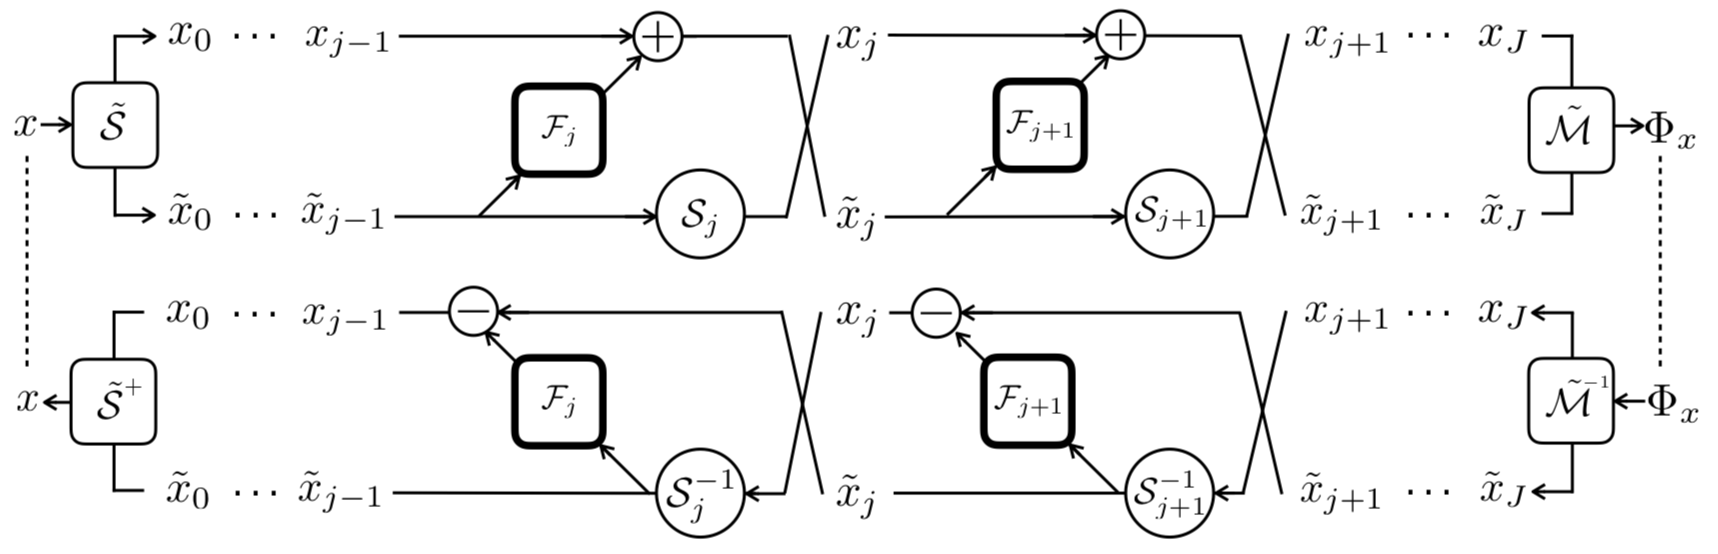
\includegraphics[width=\linewidth]{figs/i-revnet.png}
	\end{figure}
	
	\begin{figure}
		\centering
		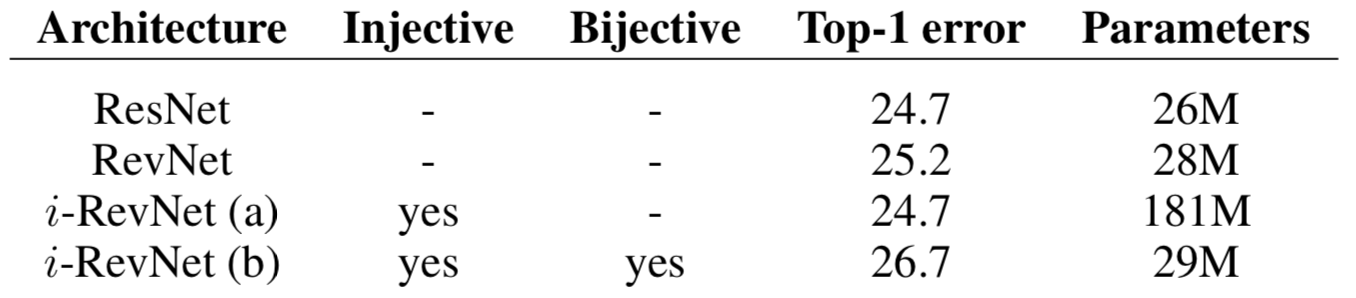
\includegraphics[width=0.9\linewidth]{figs/i-revnet_block.png}
	\end{figure}
	
	\vfill
	\hrule\medskip
	{\scriptsize \href{https://arxiv.org/pdf/1802.07088.pdf}{https://arxiv.org/pdf/1802.07088.pdf}} 
\end{frame}
%=======
\begin{frame}{References}
	{\tiny
		\begin{itemize}
			
			\item \textbf{NICE}: Non-linear Independent Components Estimation \\
			\href{https://arxiv.org/abs/1410.8516}{https://arxiv.org/abs/1410.8516} \\
			\textbf{Summary:} Uses flows to model complex high-dimensional densities. Introduce the ways to compute determinant of \\ Jacobian
			 in a simple way. Triangular Jacobian, coupling layers, factorized distribution.
			
			\item Variational Inference with Normalizing Flows \\
			\href{https://arxiv.org/abs/1505.05770}{https://arxiv.org/abs/1505.05770} \\
			\textbf{Summary:} Propose to use normalizing flows in variational inference. Discuss finite and infinitesimal flows. Uses invertible \\
			flows: planar, radial. Comparison with NICE.
			
			\item \textbf{RealNVP}: Density estimation using Real NVP \\
			\href{https://arxiv.org/pdf/1605.08803.pdf}{https://arxiv.org/pdf/1605.08803.pdf} \\
			\textbf{Summary:} Authors of NICE. The same idea and architecture, more practical. Lots of experiments and images. Coupling\\ layers with checkerboard and channel-wise permutations.
			
			\item \textbf{RevNet:} The Reversible Residual Network: Backpropagation Without Storing Activations \\
			\href{https://arxiv.org/abs/1707.04585}{https://arxiv.org/abs/1707.04585} \\
			\textbf{Summary:} RevNet allows not to store network activations. Each layer’s activations can be computed from the next layer’s activations. RevNets are composed of a series of reversible blocks. Could enable training larger and more powerful networks \\
			with limited computational resources. 
			
			\item \textbf{i-RevNet:} Deep Invertible Networks \\
			\href{https://arxiv.org/abs/1802.07088}{https://arxiv.org/abs/1802.07088} \\
			\textbf{Summary:} Invertible reversible networks. Remove noninvertible blocks (max-pooling, strides) from RevNets. Loss of \\
			information is not a necessary condition to learn representations that generalize well on hard problems, such as ImageNet.
			
		\end{itemize}
	}
\end{frame}
\end{document} 